\documentclass[fleqn,11pt]{article}
\setlength{\textwidth}{17.5cm}
\setlength{\textheight}{23.2cm}
\setlength{\hoffset}{-2.0cm}
\setlength{\voffset}{-2.5cm}

\usepackage{graphicx}
\usepackage{lastpage}
\usepackage{fancyhdr}
\usepackage{float}
\usepackage{caption}
\usepackage{subcaption}
\usepackage{color}
\usepackage[utf8]{inputenc}
\usepackage[T1]{fontenc}
\usepackage{textcomp}
\usepackage{gensymb}
\usepackage{amsmath}

\usepackage{multirow}
\usepackage{hyperref}




% list and color set.......
%%%%%%%%%%%%%%%%%%%%%%%%%%%%%%%%%%
\usepackage{color}
\usepackage{xcolor}
\usepackage{listings}
\lstloadlanguages{Matlab,Python}
\lstdefinelanguage{fei}
{morekeywords={
20NodeBrick, 27NodeBrick, 8NodeBrick, a0, a1, a2, a3, a4, acceleration, acceleration_file, acceleration_scale_unit, add, algorithm, algorithm
, all
, alpha, and, armstrong_frederick_cr, armstrong_frederick_ha, at, ax, ay, az, bending_Iy, bending_Iz, beta, beta_min, binary
, check, compressive_strength, constant, constitutive, constrain, constraint, contact_plane_vector, control, convergence, cR1, cR2, critical_stress_ratio_M, cross_section, crushing_strength, damping, databasename, define, direction, displacement, displacement_control, displacement_file, displacement_scale_unit, dof, dofs, dofs
, domain, domain
, drained, druckerprager_angle, dynamic, e0, each, eigen, Elastic_Membrane_Plate, elastic_modulus, elastic_modulus_horizontal, elastic_modulus_vertical, element, element_file, else, equal, equaldof, factor, field, filename
, fix, force_file, forces, free, friction_ratio, gamma, Gauss, h_in, help
, host, if, imposed, Imx, Imy, Imz, in, increment, initial_confining_strain, initial_confining_stress, initial_mean_pressure, integration_points, IntegrationRule, integrator, isotropic_hardening_rate, joint_1_offset, joint_2_offset, K_f, K_s, k_x, k_y, k_z, kappa, kd_in, kinematic_hardening_rate, lambda, length, linear
, load, loading, M_in, magnitude, magnitudes, mass, mass_density, master, material, maximum_gap, maximum_number_of_iterations, maximum_strain, maximum_time_step, mean, Membrane_Plate_Fiber, mesh, method, minimum_bulk_modulus, minimum_time_step, model, motion, mx, my, mz, name, new, node, nodes, nodes_file, normal_stiffness, number_of_drm_elements, number_of_drm_nodes, number_of_iterations, number_of_modes, number_of_steps, number_of_subincrements, number_of_times_reaching_maximum_strain, of, output, password, path_series, path_time_series, penalty, penalty_for_applying_generalized_displacement, point, points, poisson_ratio, poisson_ratio_h_h, poisson_ratio_h_v, porosity, port, pressure, pressure_reference_p0, print, R0, reduction, reference_void_ratio, remove, response, restore, rho_f, rho_s, rx, ry, rz
, sanisand2004_A0, sanisand2004_c, sanisand2004_ch, sanisand2004_cz, sanisand2004_ec_ref, sanisand2004_G0, sanisand2004_h0, sanisand2004_lambda_c, sanisand2004_m, sanisand2004_Mc, sanisand2004_nb, sanisand2004_nd, sanisand2004_p_cut, sanisand2004_Pat, sanisand2004_xi, sanisand2004_z_max, sanisand2008_A0, sanisand2008_alpha_cc, sanisand2008_c, sanisand2008_ch, sanisand2008_cz, sanisand2008_ec_ref, sanisand2008_G0, sanisand2008_h0, sanisand2008_K0, sanisand2008_k_c, sanisand2008_lambda, sanisand2008_m, sanisand2008_nb, sanisand2008_nd, sanisand2008_p0, sanisand2008_p_in, sanisand2008_p_r, sanisand2008_Pat, sanisand2008_rho_c, sanisand2008_theta_c, sanisand2008_X, sanisand2008_xi, sanisand2008_z_max, save, scale_factor, section, self_weight, series_file, shear, shear_modulus, shear_modulus_h_v, simple, simulate, single, slave, socket, solver, stage, state, static, steps, stiffness, stiffness_to_use, strain, strain_at_compressive_strength, strain_at_crushing_strength, strain_hardening_ratio, strain_increment_size, stress, surface, tangential_stiffness, tensile_strength, tension_softening_stiffness, test, testing, thickness, time_step, to, tolerance_1, tolerance_2, torsion_Jx, triaxial, type, undrained, unit, use, username, using, ux, uy, uz, value, variable_node_brick_8_to_27, velocity_file, velocity_scale_unit, viscoelastic_modulus, von_mises_radius, while, whos
, with, x_max, x_min, xi_in, xz_plane_vector, y_max, y_min, yield_strength, z_max, z_min},
morekeywords={[2] 20NodeBrick, 20NodeBrick_elastic, 20NodeBrick_upU, 27NodeBrick, 27NodeBrick_elastic, 27NodeBrickLT, 3NodeShell_ANDES, 4NodeShell_ANDES, 4NodeShell_MITC4, 4NodeShell_NewMITC4, 8NodeBrick, 8NodeBrick_elastic, 8NodeBrick_up, 8NodeBrick_upU, 8NodeBrickLT, beam_9dof_elastic, beam_displacement_based, beam_elastic, beam_elastic_lumped_mass, camclay, camclay_accelerated, Caughey3rd, Caughey4th, contact, DOFTYPE, druckerprager_isotropic_hardening, druckerprager_isotropic_hardening_accelerated, druckerprager_kinematic_hardening, druckerprager_kinematic_hardening_accelerated, druckerprager_perfectly_plastic, druckerprager_perfectly_plastic_accelerated, Energy_Increment, F_fluid_x, F_fluid_y, F_fluid_z, FORCETYPE, from_reactions, Fx, Fy, Fz, Hilber_Hughes_Taylor, linear, linear_elastic_crossanisotropic, linear_elastic_isotropic_3d, Modified_Newton, Mx, My, mysql, Mz, New_PisanoLT, Newmark, Newton, Norm_Displacement_Increment, Norm_Unbalance, path_series, path_time_series, pisano, pisanoLT, ProfileSPD, Rayleigh, sanisand2004, sanisand2008, static, transient, truss, UMFPack, uniaxial_concrete02, uniaxial_elastic, uniaxial_steel01, uniaxial_steel02, variable transient, vonmises_isotropic_hardening, vonmises_isotropic_hardening_accelerated, vonmises_kinematic_hardening, vonmises_kinematic_hardening_accelerated, vonmises_linear_kinematic_hardening, vonmises_linear_kinematic_hardening_accelerated, vonmises_perfectly_plastic, vonmises_perfectly_plastic_accelerated, vonmises_perfectly_plastic_LT, With_no_convergence_check,
elastic_modulus_1atm,m_in,n_in,a_in,eplcum_cr_in},
sensitive=true,
morecomment=[l]{//},
morestring=[b]",
}

\definecolor{dkgreen}{rgb}{0,0.6,0}
\definecolor{gray}{rgb}{0.5,0.5,0.5}
\definecolor{mauve}{rgb}{0.58,0,0.82}
\definecolor{ltgray}{rgb}{0.98,0.98,0.98}
\definecolor{grayish}{rgb}{0.85, 0.85, 0.85}
\lstset{language=fei, 
  frame=single,
  backgroundcolor=\color{ltgray},
  aboveskip=3mm,
  belowskip=3mm,
  showstringspaces=false,
  columns=flexible,
  basicstyle={\small\ttfamily},
  numberstyle=\tiny\color{black},
  keywordstyle=\color{blue},
  commentstyle=\color{gray},
  stringstyle=\color{mauve},
  breaklines=true,
  numbers=left,
  breakatwhitespace=true,
  tabsize=3,
  %rulecolor=\color{mauve},
}


%%%%%%%%%%%%%%%%%%%%%%%%%%%%%%%%%


\pagestyle{fancy}

\def\today
{\number\day.\space \ifcase\month\or
January\or
February\or
March\or
April\or
May\or
June\or
July\or
August\or
September\or
October\or
November\or
December\fi,\space
\number\year}

%%%%
\newcount\hh
\newcount\mm
\mm=\time
\hh=\time
\divide\hh by 60
\divide\mm by 60
\multiply\mm by 60
\mm=-\mm
\advance\mm by \time
\def\hhmm{\number\hh:\ifnum\mm<10{}0\fi\number\mm}

%%%%%
\lhead{\small \it The illustrative example for Real ESSI Simulator}
\chead{\small \it }
\rhead{\small \it \thepage{} of \pageref{LastPage} }
%
\lfoot{\small \it UC Davis}
\rfoot{\small \it \today, \hhmm}
\cfoot{\small \it Draft}
\addtolength{\headheight}{14pt}


\newcommand{\tabincell}[2]{\begin{tabular}{@{}#1@{}}#2\end{tabular}}





\begin{document}

%%%%%%%%%%%%%%%%%%%%Start Here%%%%%%%%%%%%%%%%%%%%%%%
%%%%%%%%%%%%%%%%%%%%Start Here%%%%%%%%%%%%%%%%%%%%%%%
%%%%%%%%%%%%%%%%%%%%Start Here%%%%%%%%%%%%%%%%%%%%%%%
%-------------------------------------------------------------------------------------------------------------%
%-------------------------------------------------------------------------------------------------------------%

\thispagestyle{fancy}


\tableofcontents{}








\newpage
\section{The presentation example with \emph{beam\_elastic} element}

\paragraph{Problem description:} ~

\begin{itemize}
  \item Structure size

    Structure Width=6m, Height=6m, Force=100N 

  \item Element size

    Element length=6m, width=1m, height=1m, $\rho=0.0$, E=1E8Pa, $\nu=0.0$.
\end{itemize}


\begin{figure}[H]
  \centering
  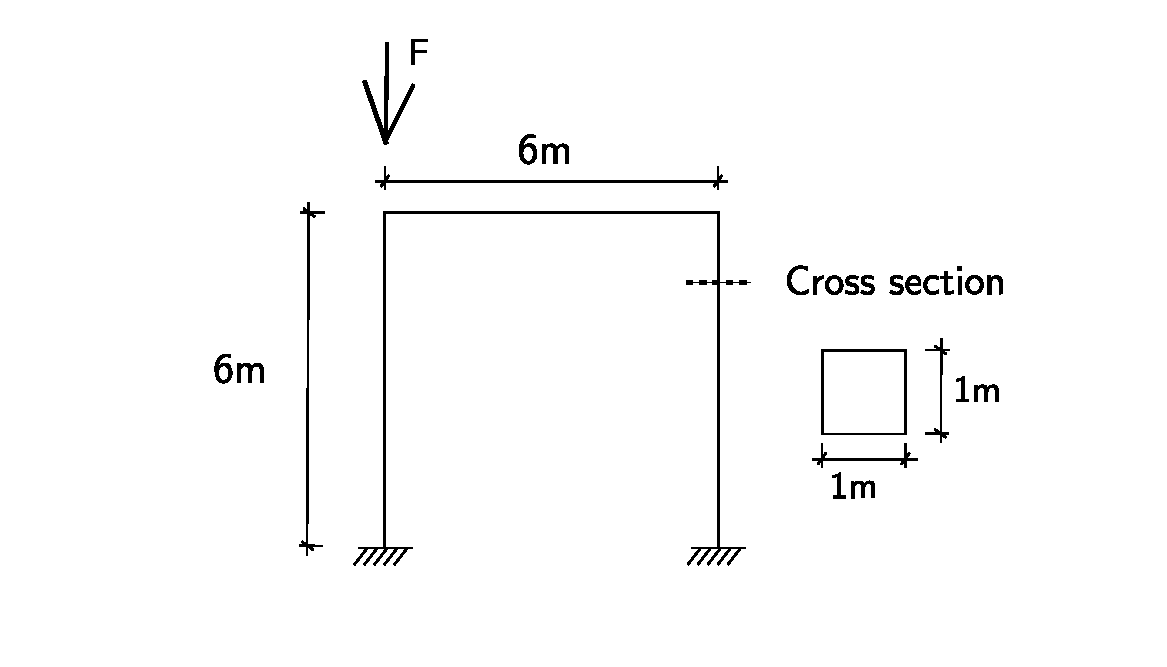
\includegraphics[width=12cm]{../Figure-files/beam_elastic_frame_descrip.pdf}
  \caption{Problem description for the presentation example with \emph{beam\_elastic} element}
  \label{fig Problem description for the presentation example with beam element}
\end{figure}





\paragraph{ESSI model fei file: } ~

\lstinputlisting[frame=single]{../Figure-files/1beam_elastic_presentation.fei}

The ESSI model fei files for this example can be downloaded \href{https://github.com/yuan-energy/Real-ESSI-Examples/blob/master/model_fei_file/beam_elastic_presentation_example/beam_elastic_presentation_example.tgz?raw=true}{here}.














\newpage
\section{ShearBeam Element for Pisano Materials}

\paragraph{Problem description:} ~

In the element type "ShearBeamLT", only one Gauss point exists. So the one ShearBeamLT element was used here to test the Pisano\footnote{Federico Pisanò and Boris Jeremić. Simulating stiffness degradation and damping in soils via a simple
visco-elastic–plastic model. Soil Dynamics and Earthquake Engineering, 63:98–109, 2014} materials. 

As shown in the figure (\ref{fig ShearBeam element to test the plastic materials}), only one Gauss point exists in the middle of ShearBeam element. The vertical force $F_z$ was used as the confinement for the Gauss point. And the back and forth force $F_x$ was used as loading and unloading for the Gauss point. 

\begin{figure}[H]
  \centering
  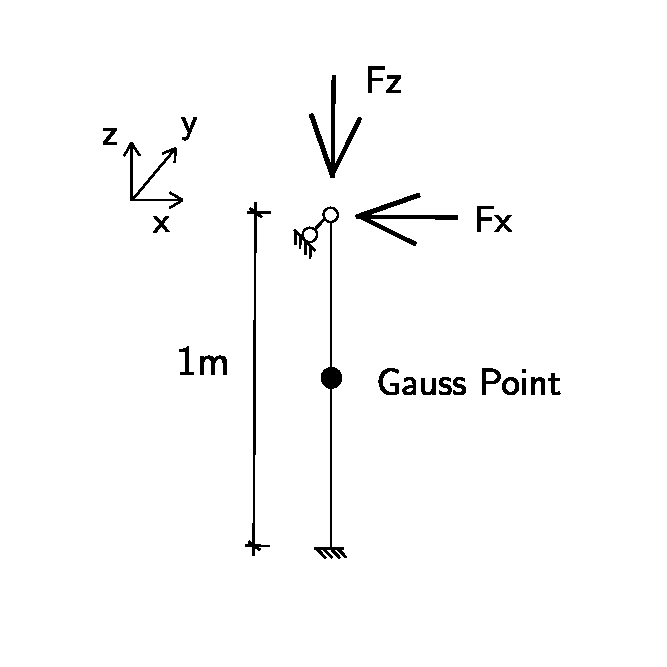
\includegraphics[width=10cm]{../Figure-files/pisano_descrip.pdf}
  \caption{ShearBeam element to test the plastic materials}
  \label{fig ShearBeam element to test the plastic materials}
\end{figure}

\newpage
\paragraph{Results} ~

The stress-strain relationship was plotted in Fig.(\ref{fig Shear stress-strain relationship in the Pisano model}). 

\begin{figure}[H]
  \centering
  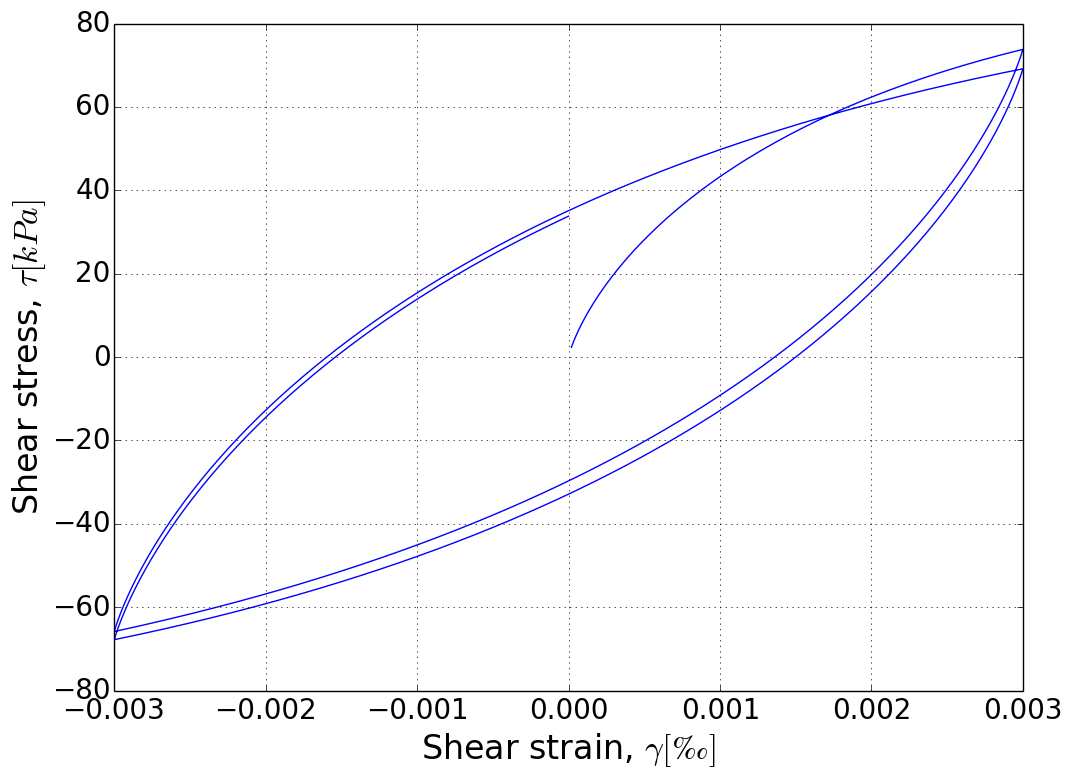
\includegraphics[width=12cm]{../Figure-files/pisanoLT_test01.png}
  \caption{Shear stress-strain relationship in the Pisano model}
  \label{fig Shear stress-strain relationship in the Pisano model}
\end{figure}

\paragraph{ESSI model fei file: } ~

\lstinputlisting[frame=single]{../Figure-files/2test_pisano_01.fei}

The ESSI model fei files for this example can be downloaded \href{https://github.com/yuan-energy/Real-ESSI-Examples/blob/master/model_fei_file/shearbeam_pisano_plastic/shearbeam_pisano_plastic.tgz?raw=true}{here}.









\newpage
\section{4NodeANDES cantilever beams under the force perpendicular to plane}

\paragraph{Problem description:} ~

Length=6m, Width=1m, Height=1m, Force=100N, E=1E8Pa, $\nu=0.0$. 

\begin{figure}[H]
  \centering
  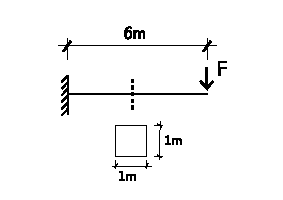
\includegraphics[width=7cm]{../Figure-files/cantilever_6.pdf}
  \caption{Problem description for cantilever beams}
  \label{fig Problem description for cantilever 4}
\end{figure}


\paragraph{Numerical model:} ~

\vskip 12pt

When the force direction is perpendicular to the plane, only the bending deformation is calculated in 4NodeANDES elements. 


The 4NodeANDES elements were shown in Figure (\ref{fig 4NodeANDES elements for cantilever beams under force perpendicular to plane}).

\begin{figure}[H]
  \centering
  \begin{subfigure}{0.5\textwidth}
    \centering
    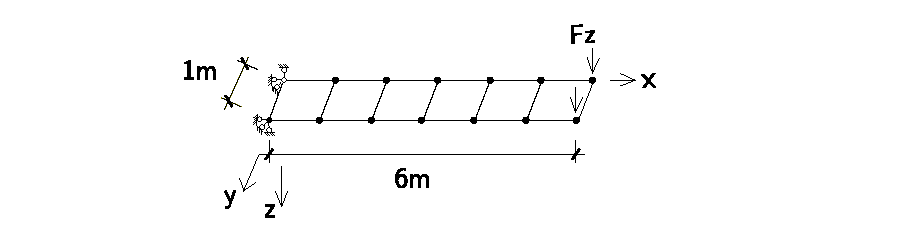
\includegraphics[width=10cm]{../Figure-files/beam_ANDES_xy_bending_6div.pdf}
    % \caption{Six 4NodeANDES elements}
  \end{subfigure}
  \captionsetup{justification=centering,margin=3cm}
  \caption{4NodeANDES elements for cantilever beams under force perpendicular to plane}
  \label{fig 4NodeANDES elements for cantilever beams under force perpendicular to plane}
\end{figure}


\paragraph{ESSI model fei file: } ~

\lstinputlisting[frame=single]{../Figure-files/3_perpend_ANDES.fei}

The ESSI model fei files for this example can be downloaded \href{https://github.com/yuan-energy/Real-ESSI-Examples/blob/master/model_fei_file/ANDESshell_cantilever_perpendicular_to_plane/ANDESshell_cantilever_perpendicular_to_plane.tgz?raw=true}{here}.








\newpage
\section{4NodeANDES cantilever beams under the inplane force}

\paragraph{Problem description:} ~

Length=6m, Width=1m, Height=1m, Force=100N, E=1E8Pa, $\nu=0.0$. 

\begin{figure}[H]
  \centering
  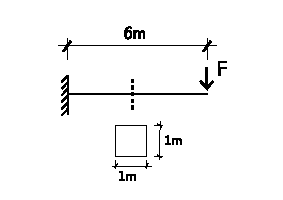
\includegraphics[width=7cm]{../Figure-files/cantilever_6.pdf}
  \caption{Problem description for cantilever beams}
  \label{fig Problem description for cantilever 4 2}
\end{figure}

\paragraph{Numerical model:} ~

When the force direction is inplane, both the bending and shear deformation are calculated in 4NodeANDES elements. 

The 4NodeANDES elements under inplane force were shown in Figure (\ref{fig 4NodeANDES elements for cantilever beams under inplane force}).

\begin{figure}[H]
  \centering
  \vskip 8pt
  \begin{subfigure}{0.5\textwidth}
    \centering
    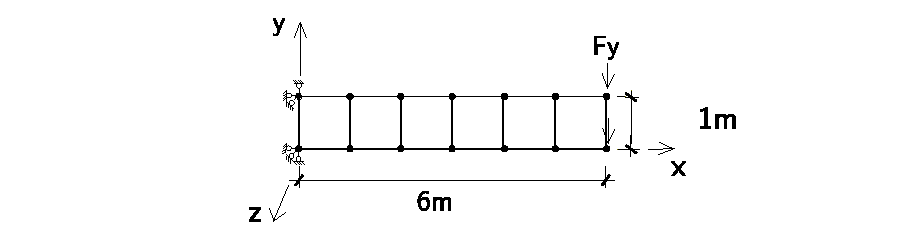
\includegraphics[width=10cm]{../Figure-files/beam_ANDES_yz_inPlane_6div.pdf}
  \end{subfigure}
  \captionsetup{justification=centering,margin=3cm}
  \caption{4NodeANDES elements for cantilever beams under inplane force}
  \label{fig 4NodeANDES elements for cantilever beams under inplane force}
\end{figure}


\paragraph{ESSI model fei file: } ~

\lstinputlisting[frame=single]{../Figure-files/4_inplane_ANDES.fei}


The ESSI model fei files for this example can be downloaded \href{https://github.com/yuan-energy/Real-ESSI-Examples/blob/master/model_fei_file/ANDESshell_cantilever_inplane/ANDESshell_cantilever_inplane.tgz?raw=true}{here}.








\newpage
\section{27NodeBrick cantilever beam for different Poisson's ratio}

\paragraph{Problem description: } ~

Length=6m, Width=1m, Height=1m, Force=100N, E=1E8Pa, $\nu=0.0-0.49$.
The force direction was shown in Figure (\ref{fig Problem description for cantilever beams of different Poisson's 27}). 

\begin{figure}[H]
  \centering
  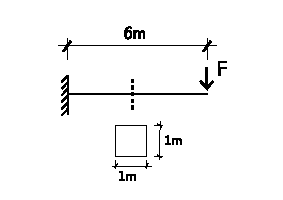
\includegraphics[width=7cm]{../Figure-files/cantilever_6.pdf}
  \caption{Problem description for cantilever beams of different Poisson's ratios}
  \label{fig Problem description for cantilever beams of different Poisson's 27}
\end{figure}

\paragraph{Numerical model:} ~

The 27NodeBrick elements for cantilever beams of different Poisson's ratios were shown in Figure (\ref{fig 27NodeBrick elements for cantilever beams of different Poisson's ratios}):
\begin{figure}[H]
  \centering
  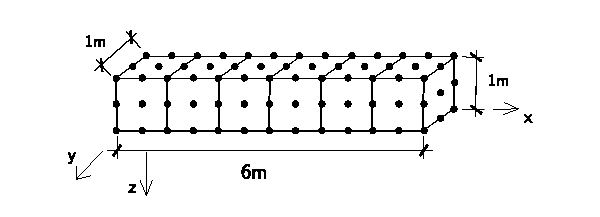
\includegraphics[width=9cm]{../Figure-files/beam_27brick_6div.pdf}
  \caption{27NodeBrick elements for cantilever beams of different Poisson's ratios}
  \label{fig 27NodeBrick elements for cantilever beams of different Poisson's ratios}
\end{figure}

\paragraph{ESSI model fei file: } ~

This is a model fei for just one Poisson's ratio value.

\lstinputlisting[frame=single]{../Figure-files/5_27NodeBrick.fei}

The ESSI model fei files for this example can be downloaded \href{https://github.com/yuan-energy/Real-ESSI-Examples/blob/master/model_fei_file/27NodeBrick_cantilever_different_Poisson/27NodeBrick_cantilever_different_Poisson.tgz?raw=true}{here}.









\newpage
\section{27NodeBrick cantilever beams for dynamic input}



\paragraph{Problem description:} ~



Length=20m, Width=1m, Height=1m, E=504MPa, $\nu=0.4$. 

All degree of freedoms at the bottom nodes are fixed. 

The load was a dynamic input. 


\begin{figure}[H]
  \centering
  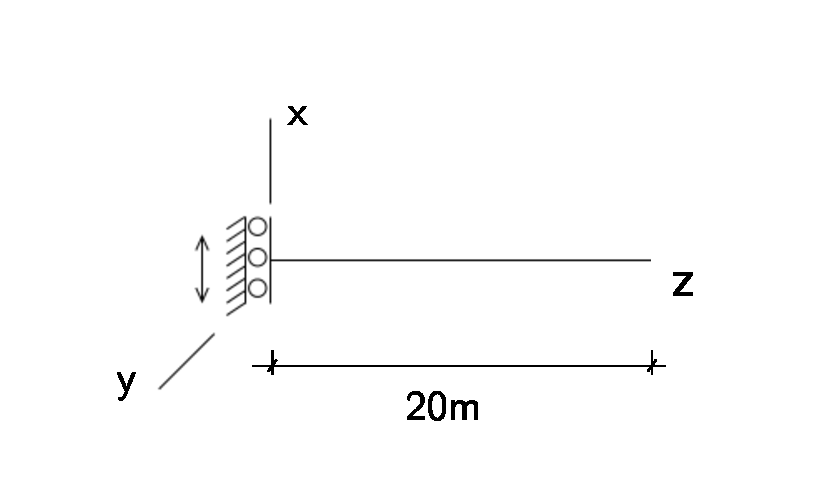
\includegraphics[width=8cm]{../Figure-files/dynamic_example_diagram.pdf}
  \caption{Problem description for one simple dynamic example}
  \label{fig Problem description for one simple dynamic example}
\end{figure}



\paragraph{Numerical model:} ~

The numerical model applied 27NodeBrick to simulate the 1D motion. 

\begin{figure}[H]
  \centering
  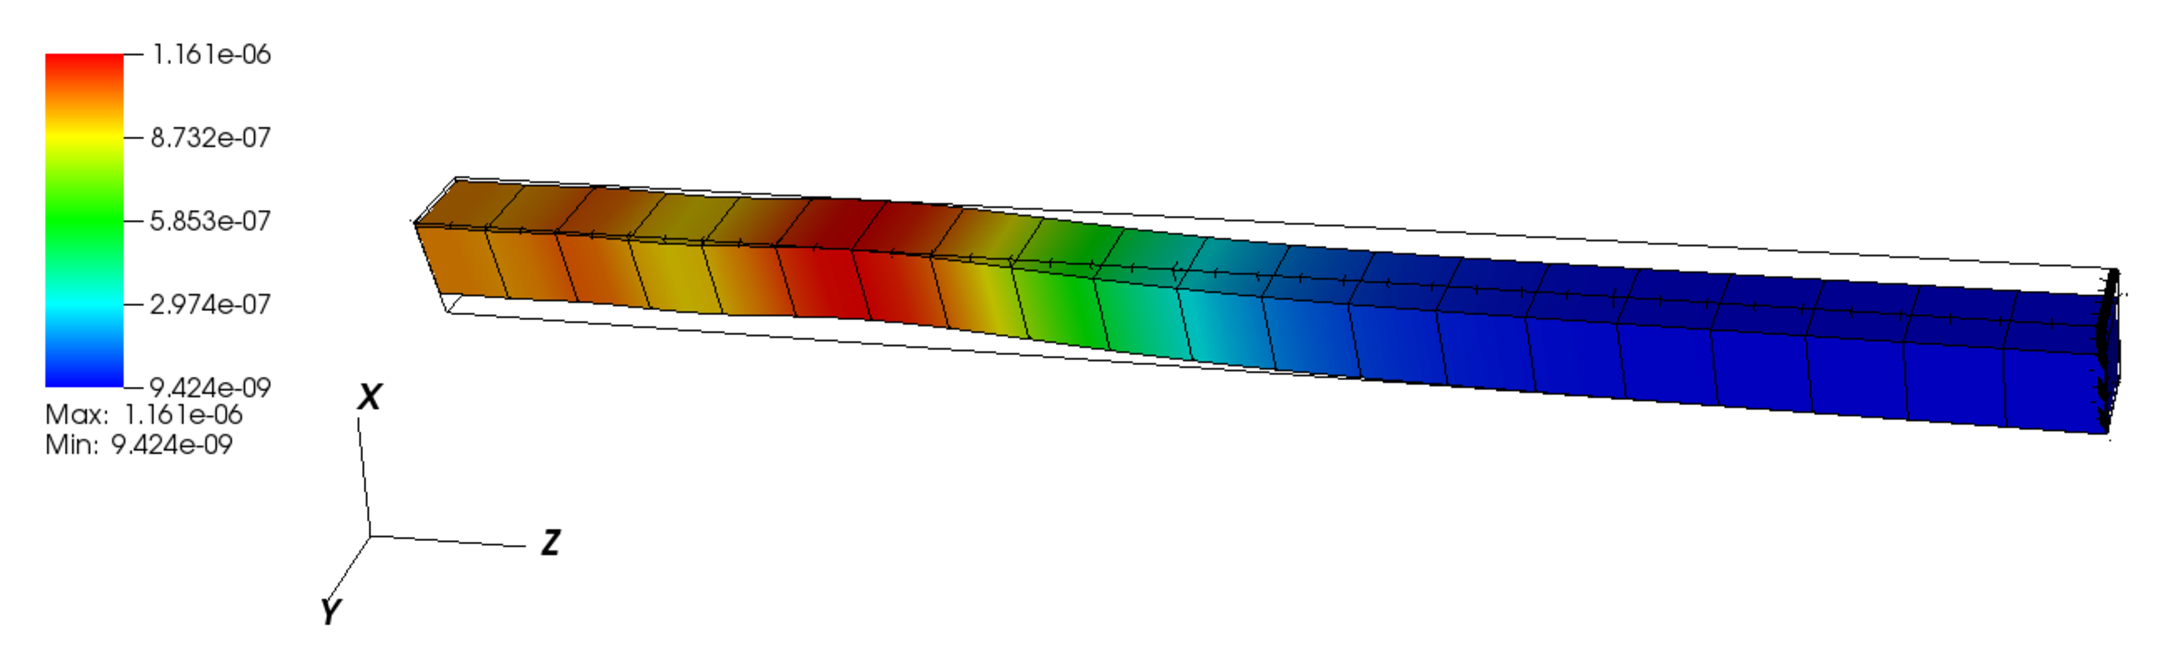
\includegraphics[width=16cm]{../Figure-files/dynamic_example_numerical.pdf}
  \caption{Numerical model for one simple dynamic example}
  \label{fig Numerical model for one simple dynamic example}
\end{figure}

\paragraph{ESSI model fei file: } ~

\lstinputlisting[frame=single]{../Figure-files/6dynamic_example.fei}


The ESSI model fei files for this example can be downloaded \href{https://github.com/yuan-energy/Real-ESSI-Examples/blob/master/model_fei_file/27NodeBrick_dynamic_impose_motion/27NodeBrick_dynamic_impose_motion.tgz?raw=true}{here}.











\newpage
\section{4NodeANDES square plate with four edges clamped}



\paragraph{Problem description:} ~



Length=20m, Width=20m, Height=1m, Force=100N, E=1E8Pa, $\nu=0.3$. 

The four edges are \textbf{clamped}. 

The load is the uniform normal pressure on the whole plate. Self weight is used to apply the uniform normal pressure. 


\begin{figure}[H]
  \centering
  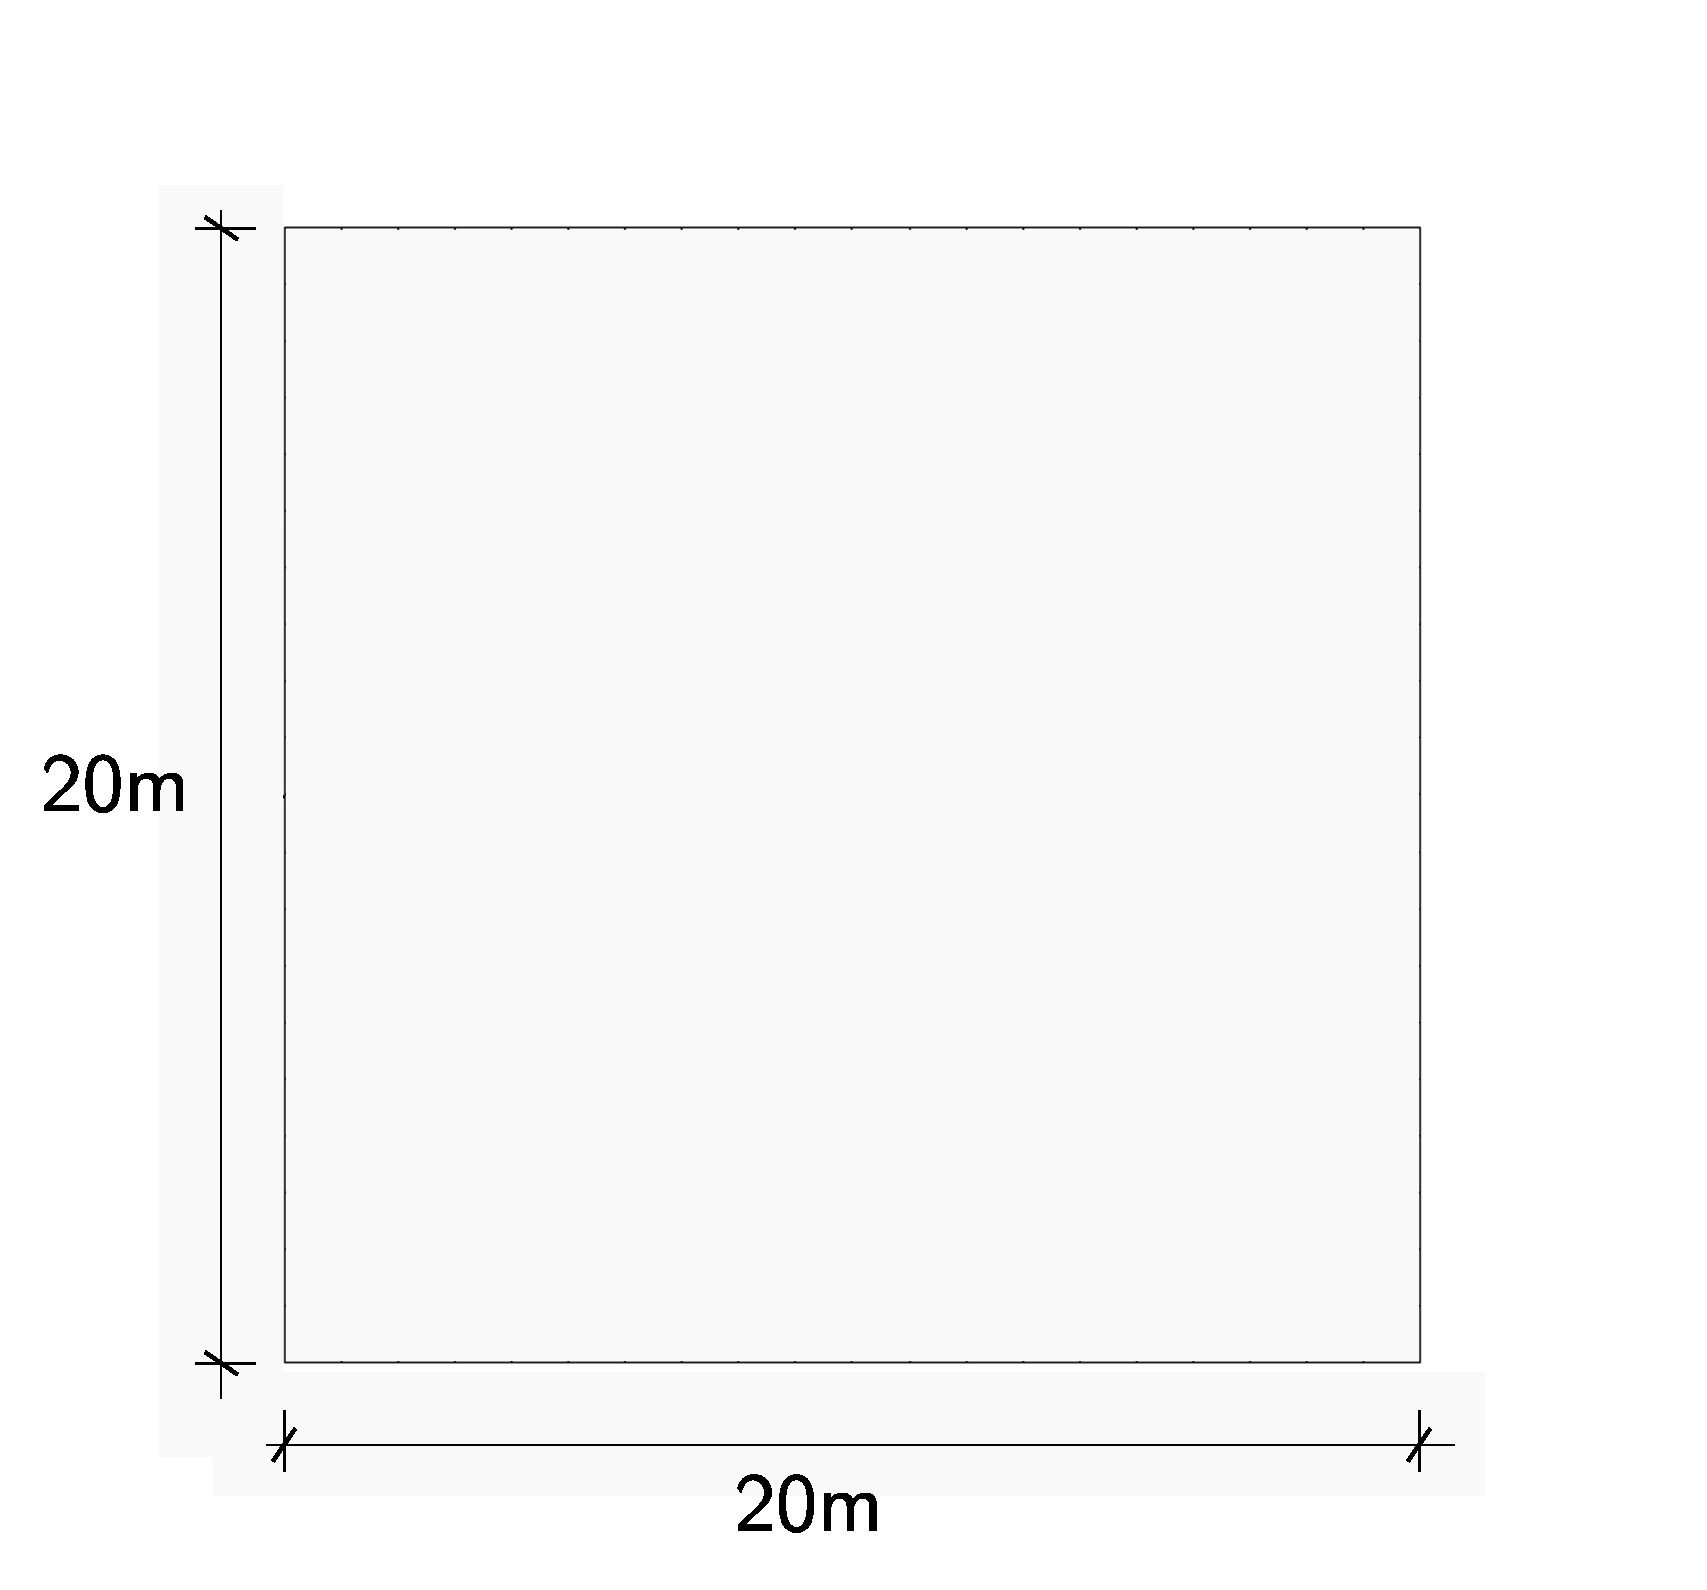
\includegraphics[width=10cm]{../Figure-files/square_plate_descrp.pdf}
  \caption{Square plate with four edges clamped }
  \label{fig 4NodeANDES edges clamped square plate with element side length for program description }
\end{figure}


\newpage
\paragraph{Numerical model:} ~

The element side length is 1 meter. 


\begin{figure}[H]
  \centering
  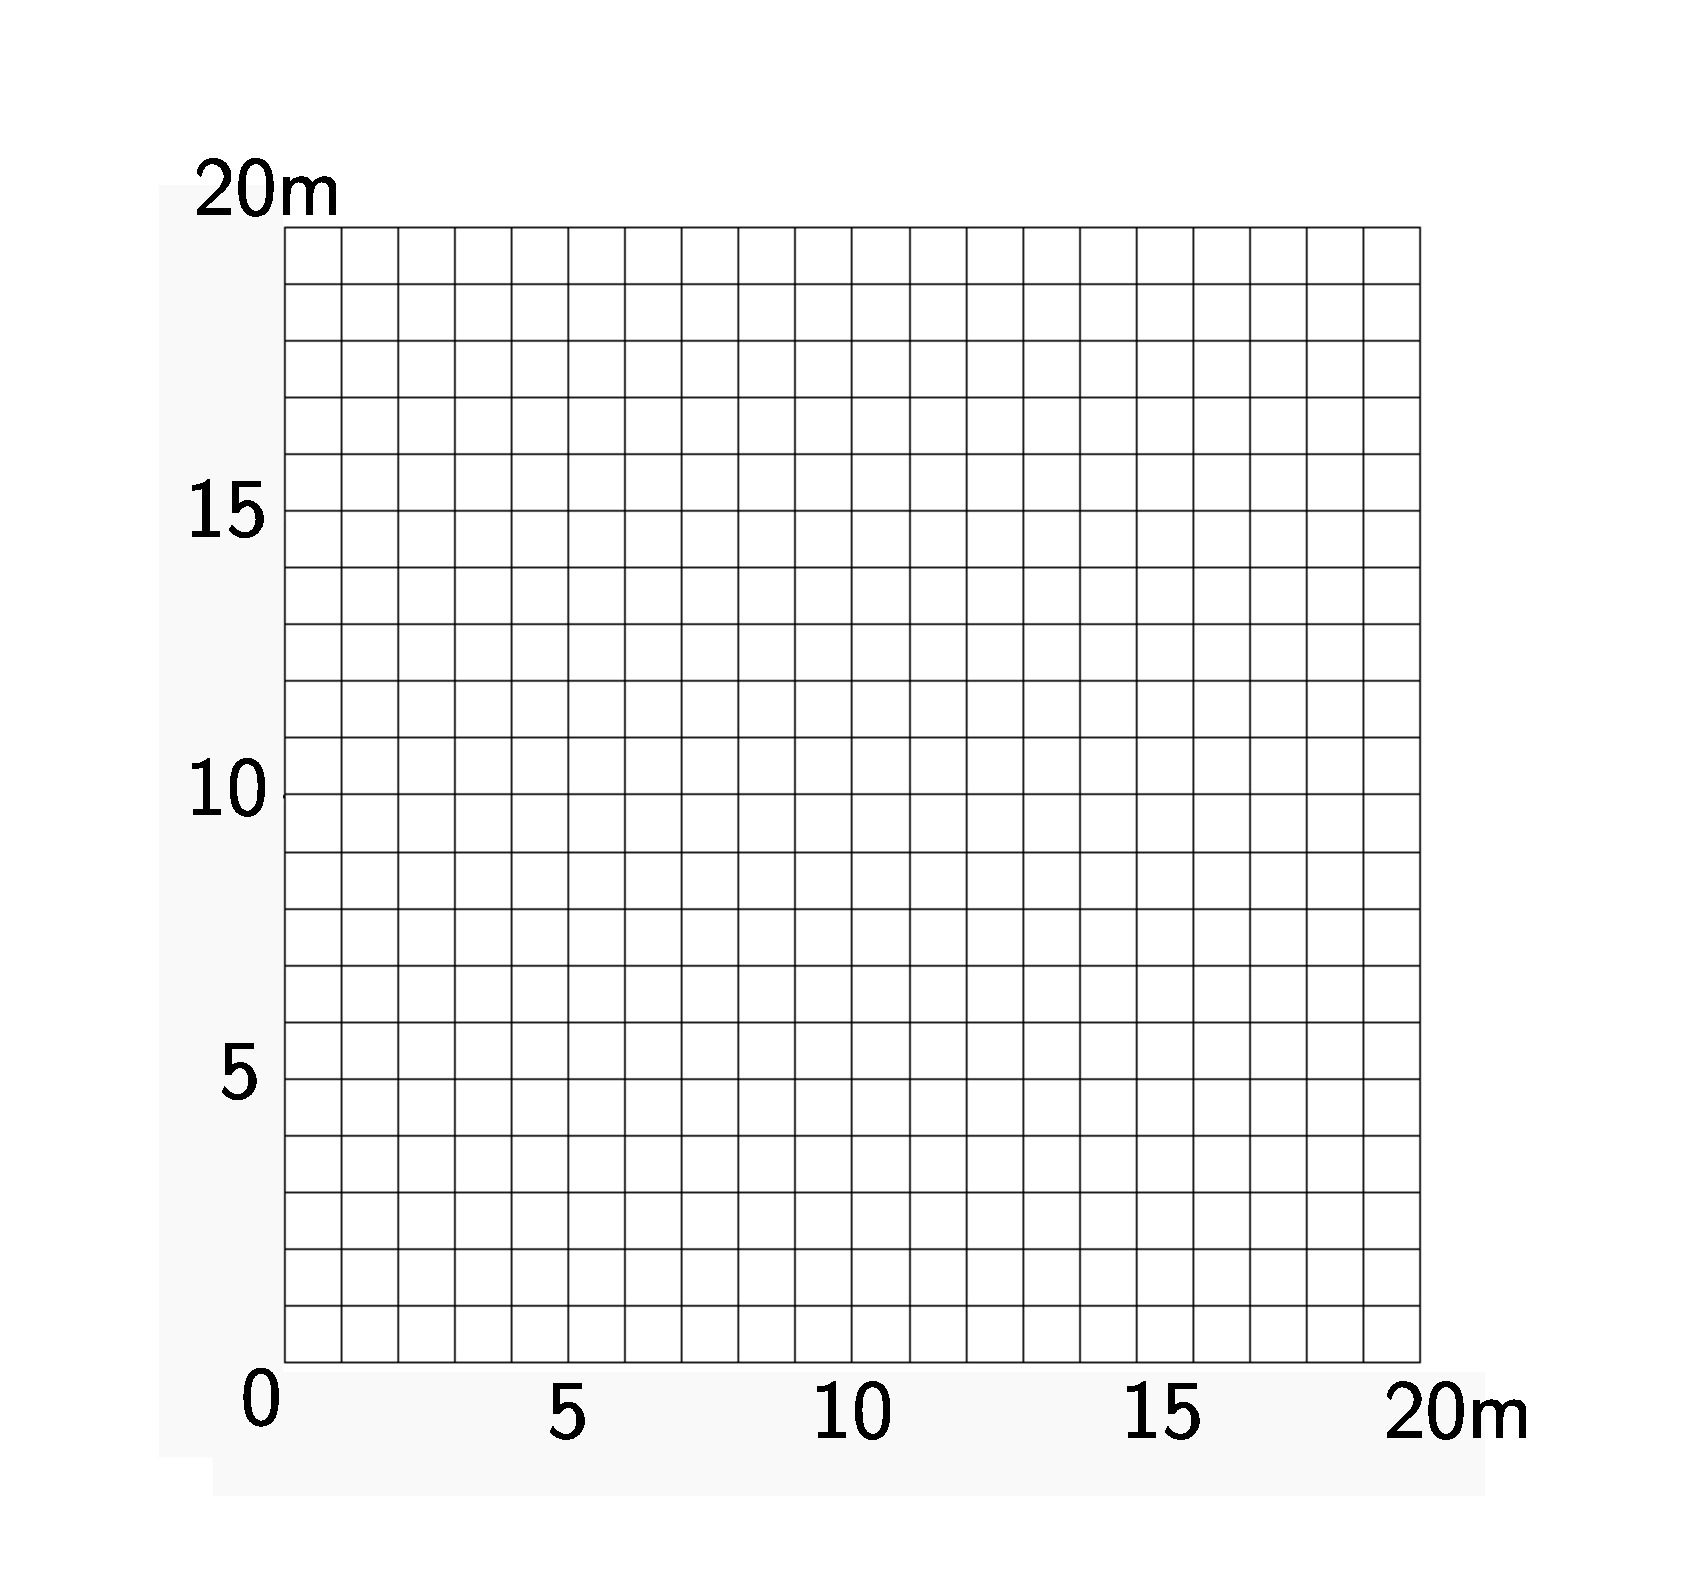
\includegraphics[width=10cm]{../Figure-files/square_plate4_2.pdf}
  \caption{4NodeANDES edge clamped square plate with element side length 1m }
  \label{fig 4NodeANDES edges clamped square plate with element side length 1m }
\end{figure}


\paragraph{ESSI model fei file: } ~

\lstinputlisting[frame=single]{../Figure-files/7shell.fei}


The ESSI model fei files for this example can be downloaded \href{https://github.com/yuan-energy/Real-ESSI-Examples/blob/master/model_fei_file/ANDESshell_square_plate/ANDESshell_square_plate.tgz?raw=true}{here}.




















\newpage
\section{Domain Reduction Method (DRM) in ESSI}


Domain Reduction Method (DRM) is a finite element methodology for modeling earthquake ground motion. Please look at the reference\footnote{Bielak, J., Loukakis, K., Hisada, Y., and Yoshimura, C. (2003). Domain reduction method for three-dimensional earthquake modeling in localized regions, Part I: Theory. Bulletin of the Seismological Society of America, 93(2), 817-824.} for more information. 

\subsection{One dimensional DRM model with 8NodeBrickLT element}

\paragraph{Problem description:} ~


One simple 1D DRM model is shown in Fig.(\ref{fig Program description for the 1D DRM model}). The "DRM element", "Exterior node" and "Boundary node" are required to be designated in the DRM HDF5 input. The format and script for the HDF5 input are shown in Appendix.A. 

\begin{figure}[H]
  \centering
  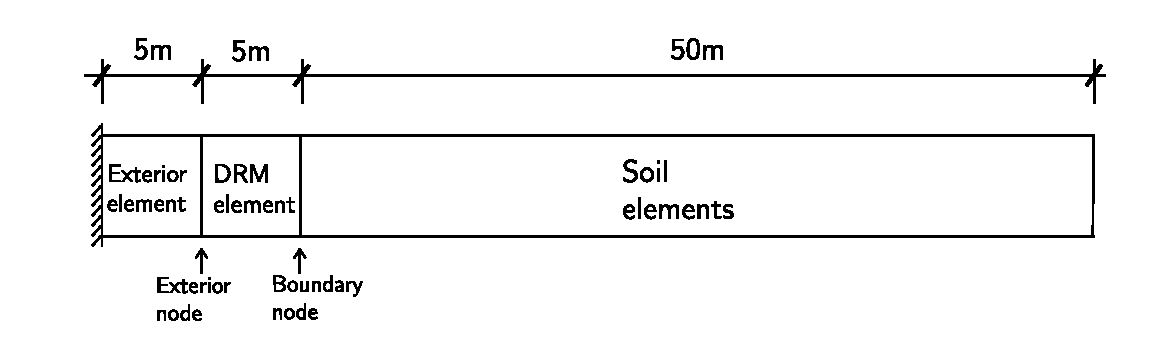
\includegraphics[width=18cm]{../Figure-files/DRM_1D_descrp.pdf}
  \caption{Program description for the 1D DRM model}
  \label{fig Program description for the 1D DRM model}
\end{figure}




\paragraph{Numerical model:} ~


\begin{figure}[H]
  \centering
  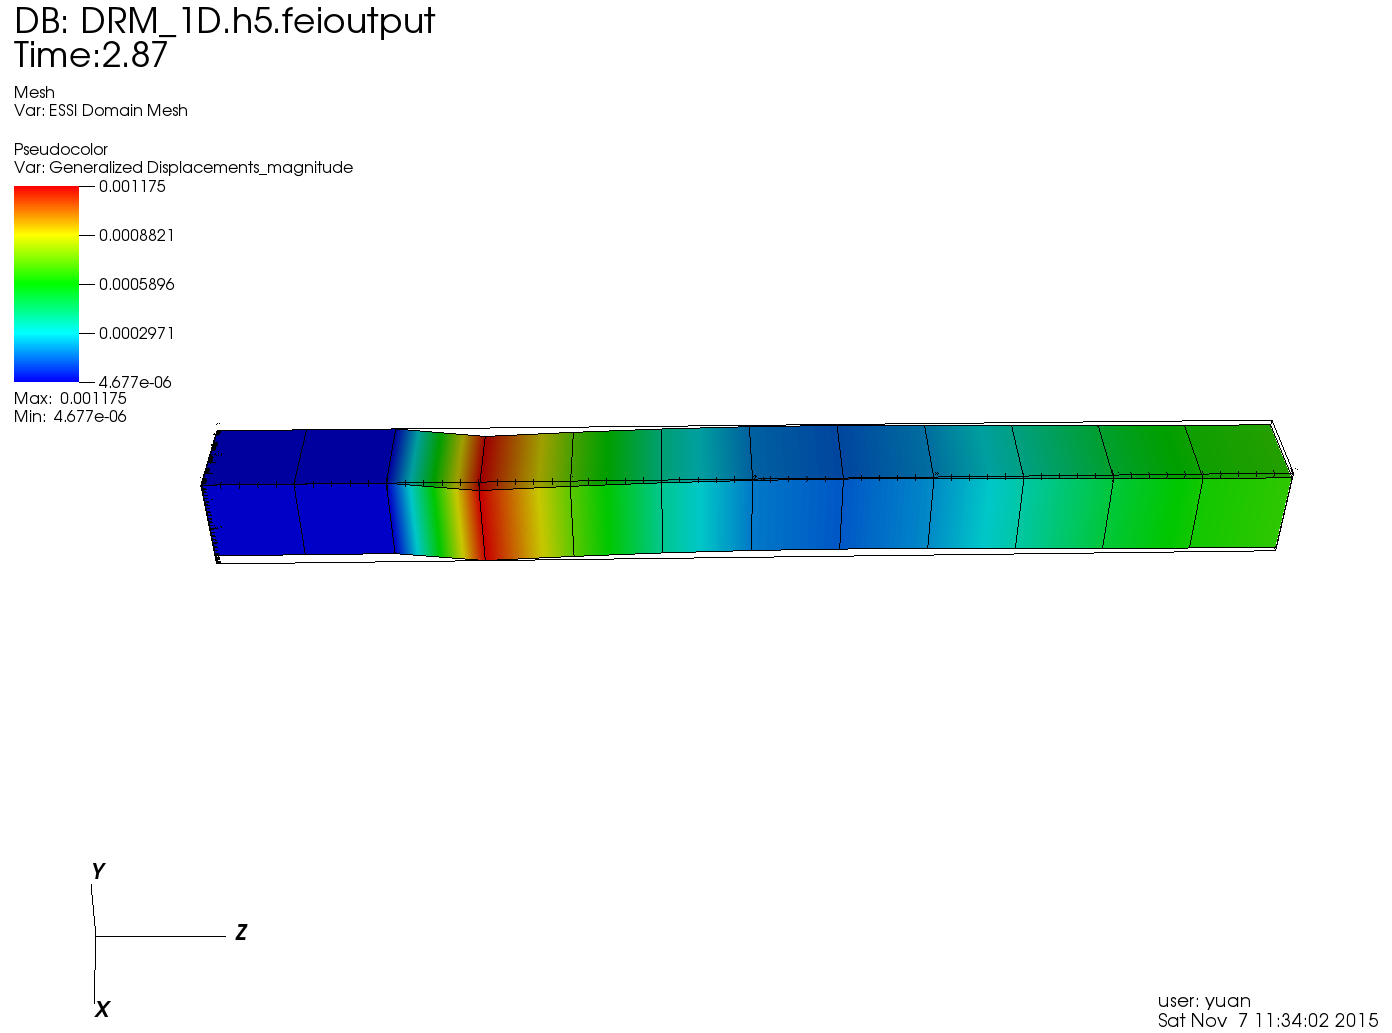
\includegraphics[width=15cm]{../Figure-files/DRM_1D_result41.png}
  \caption{Diagram for the 1D DRM model}
  \label{fig Diagram for the 1D DRM model}
\end{figure}




\paragraph{ESSI model fei file: } ~

\lstinputlisting[frame=single]{../Figure-files/DRM_1D_script.fei}

The ESSI model fei files for this example can be downloaded \href{https://github.com/yuan-energy/Real-ESSI-Examples/blob/master/model_fei_file/DRM_1D/DRM_1D.tgz?raw=true}{here}.






\vskip 20pt
\subsection{Three dimensional DRM model with 8NodeBrickLT element}

\paragraph{Problem description:} ~

As shown in Fig.(\ref{fig The diagram for Domain Reduction Method DRM }), the DRM layer is used to add the earthquake motion. 


\begin{figure}[H]
  \centering
  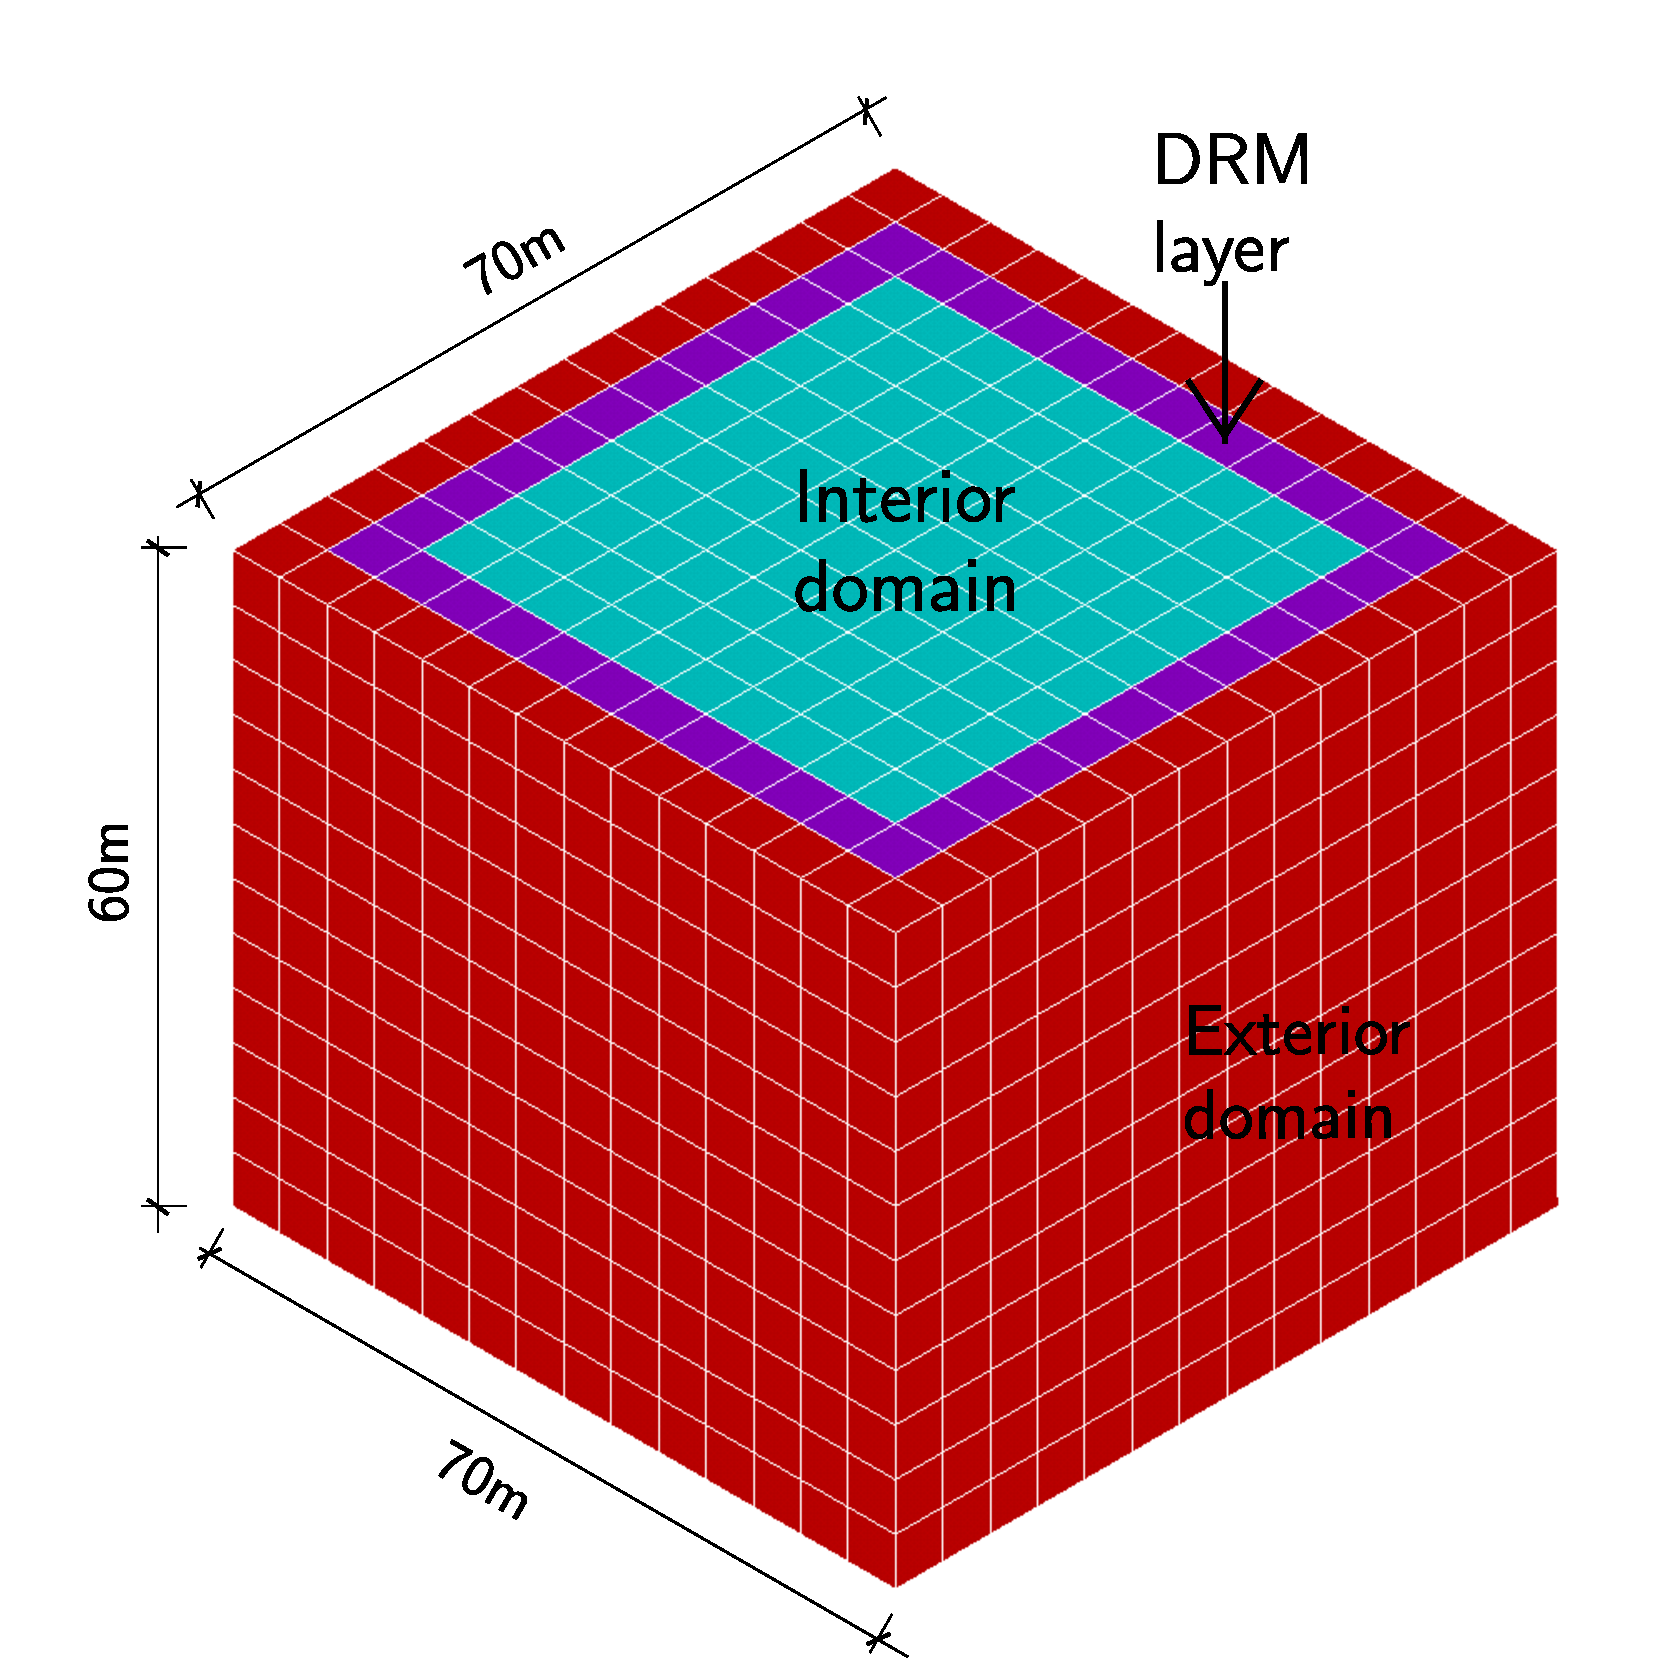
\includegraphics[width=10cm]{../Figure-files/DRM_3D_descp_3.pdf}
  \caption{The diagram for 3D Domain Reduction Method (DRM) }
  \label{fig The diagram for Domain Reduction Method DRM }
\end{figure}


% In 2D, the DRM model is shown in Fig.(\ref{fig The diagram for Domain Reduction Method DRM 2d }). 
% \begin{figure}[H]
%   \centering
%   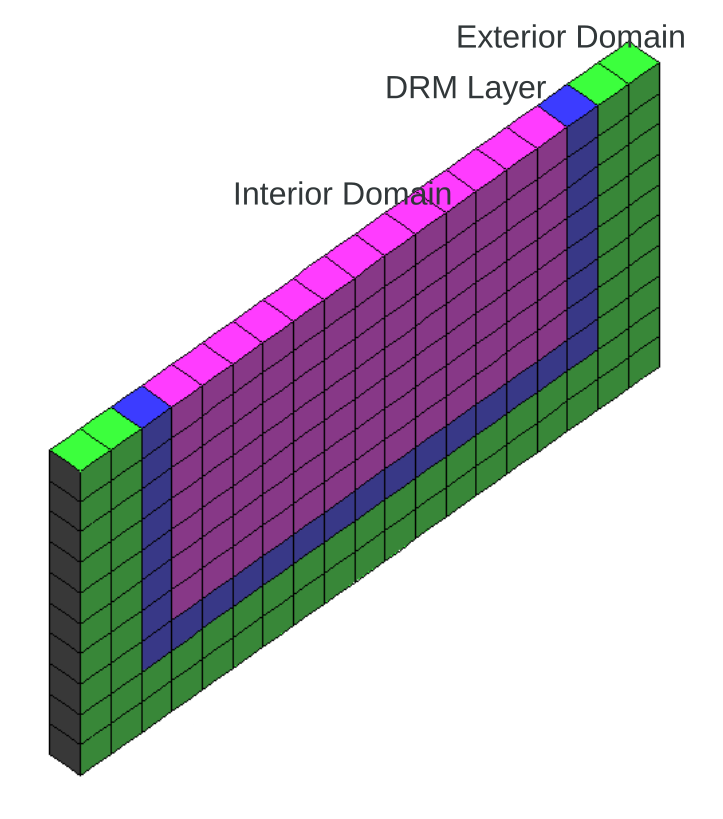
\includegraphics[width=10cm]{../Figure-files/DRM_diagram_2d.png}
%   \caption{The diagram for 2D Domain Reduction Method (DRM) }
%   \label{fig The diagram for Domain Reduction Method DRM 2d }
% \end{figure}




\paragraph{Numerical result:} ~

\begin{figure}[H]
  \centering
  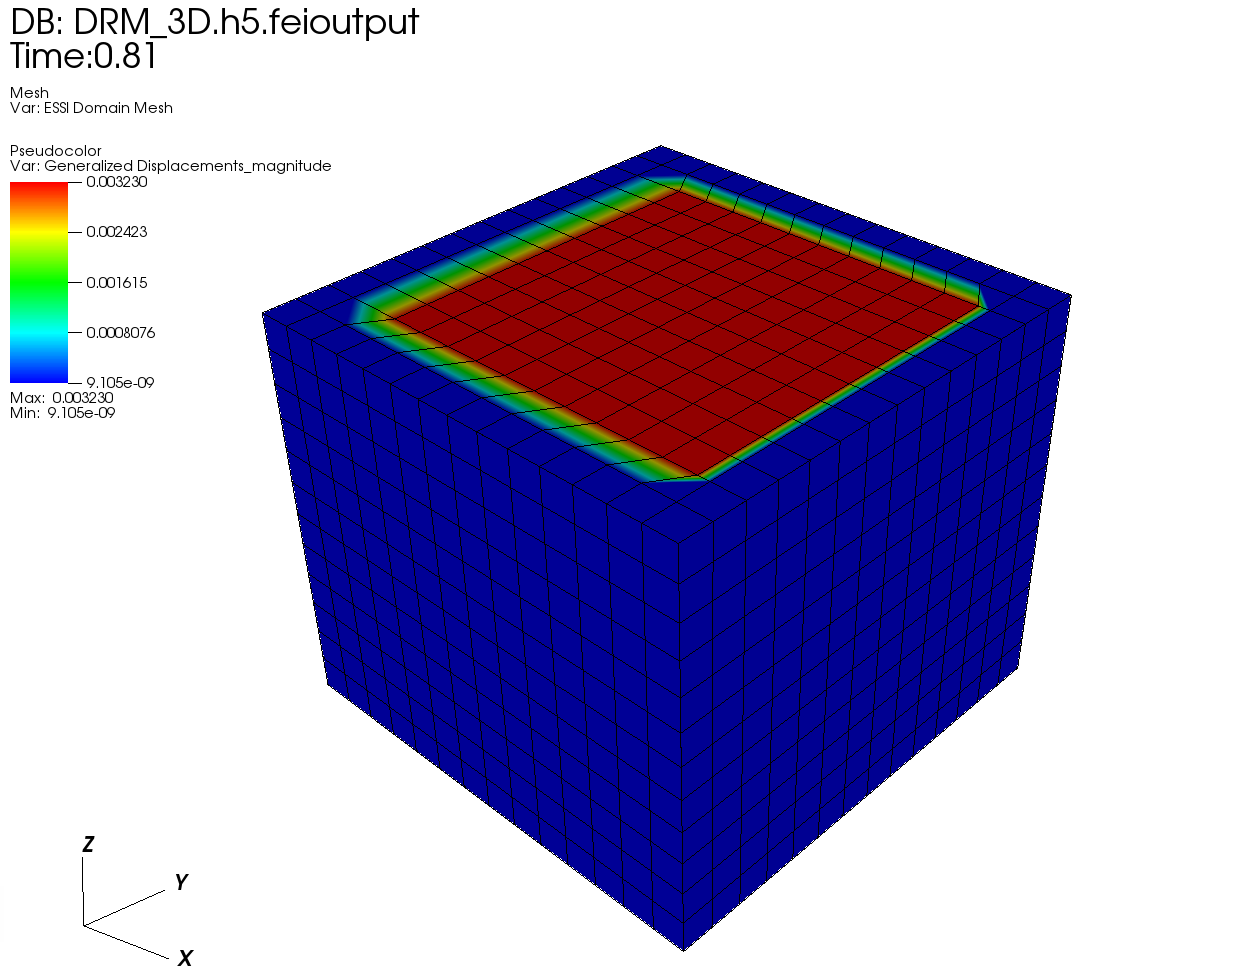
\includegraphics[width=15cm]{../Figure-files/3d_drm_result429.png}
  \caption{Diagram for the 3D DRM model}
  \label{fig Diagram for the 3D DRM model}
\end{figure}


\paragraph{ESSI model fei file: } ~

\lstinputlisting[frame=single]{../Figure-files/DRM_3D_script.fei}

The ESSI model fei files for this example can be downloaded \href{https://github.com/yuan-energy/Real-ESSI-Examples/blob/master/model_fei_file/DRM_3D/DRM_3D.tgz?raw=true}{here}.






\newpage
\section{References}
\nocite{*}
\bibliographystyle{plain}
\bibliography{reference}


\newpage
\section{Appendix}

\paragraph{Appendix.A \\
How to make the DRM input in HDF5 format?} ~


As shown in Fig.(\ref{fig The HDF5 format for DRM input}), eight things are required in the DRM input. 

\begin{figure}[H]
  \centering
  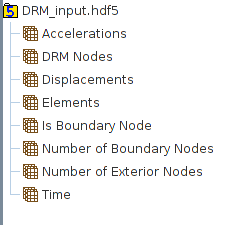
\includegraphics[width=7cm]{../Figure-files/DRM_input_format.png}
  \caption{The HDF5 format for DRM input}
  \label{fig The HDF5 format for DRM input}
\end{figure}

The name of the subfolders must be exactly same with the name designated here.

\begin{enumerate}
  \item Elements. 
  
  Elements are the element number of DRM elements, which are used to add the earthquake motion. 

  \item DRM Nodes. 
  
  DRM Nodes are the node number of the DRM elements. 

  \item Is Boundary Node. 

  "Is Boundary Node" is used to describe that whether the nodes in "DRM Nodes" are the boundary nodes or the exterior nodes.

  If this value is "1", the corresponding node in "DRM Nodes" is a boundary node.

  If this value is "0", the corresponding node in  "DRM Nodes" is an exterior node in the DRM element.

  \item Number of Boundary Nodes. 

  This is the number of boundary nodes.

  \item Number of Exterior Nodes. 

  This is the number of exterior nodes.

  \item Displacements. 

  Displacements are the displacement components of the input earthquake motion on the corresponding DRM Nodes. Displacements are a 2D array, in which the column number is the timestep number. And each row represents the displacement in one direction. If every node has 3 degrees of freedom (DOFs) in terms of ux, uy, and uz, the first three rows represent the input displacements on the first DRM node in the directions of ux, uy, and uz. Then, the next three rows represent the input displacements for the next node. So the total row number should be three times of the number of DRM Nodes.

  \item Accelerations. 

  Accelerations have the same data structure with the displacements. 
  
  \item Time. 

  This is the real time for each timestep in the input earthquake motion. 


\end{enumerate}

\paragraph{Python and Matlab script to generate the DRM HDF5-based input} ~

You can either use Python or Matlab to generate the DRM HDF5-based input.  

Python script:
\lstinputlisting[language=Python, frame=single]{../Figure-files/generate_hdf5_drm_input.py}


\newpage
\textbf{Matlab script:}

This is a matlab function to write DRM input in HDF5 format. 

ESSI-users need to define the function arguments (e.g."time", "DRMelement") by themselves according to the actual model. 

\lstinputlisting[language=Matlab, frame=single]{../Figure-files/write_DRM_hdf5.m}

The Python and Matlab script files can be downloaded \href{https://github.com/yuan-energy/Real-ESSI-Examples/blob/master/model_fei_file/Script_to_Generate_DRM_input/Script_to_Generate_DRM_input.tgz?raw=true}{here}.





%-------------------------------------------------------------------------------------------------------------%
%-------------------------------------------------------------------------------------------------------------%

\end{document}


        10        20        30        40        50        60        70        80
12345678901234567890123456789012345678901234567890123456789012345678901234567890
